\documentclass[a4paper,10pt]{article}
\usepackage[utf8]{inputenc}

% ******************************************************************************
% ****************************** Custom Margin *********************************

% Add `custommargin' in the document class options to use this section
% Set {innerside margin / outerside margin / topmargin / bottom margin}  and
% other page dimensions

\ifsetMargin
\else
    \RequirePackage[left=37mm,right=30mm,top=35mm,bottom=30mm]{geometry}
    \setFancyHdr % To apply fancy header after geometry package is loaded
\fi

% *****************************************************************************
% ******************* Fonts (like different typewriter fonts etc.)*************

% Add `customfont' in the document class option to use this section

\ifsetFont
\else
    % Set your custom font here and use `customfont' in options. Leave empty to
    % load computer modern font (default LaTeX font).  

    \RequirePackage{libertine} 
\fi

% *****************************************************************************
% **************************** Custom Packages ********************************


% ************************* Algorithms and Pseudocode **************************

%\usepackage{algpseudocode} 


% ********************Captions and Hyperreferencing / URL **********************

% Captions: This makes captions of figures use a boldfaced small font. 
%\RequirePackage[small,bf]{caption}

\RequirePackage[labelsep=space,tableposition=top]{caption} 
\renewcommand{\figurename}{Fig.} %to support older versions of captions.sty

% ************************ Formatting / Footnote *******************************

%\usepackage[perpage]{footmisc} %Range of footnote options 


% ****************************** Line Numbers **********************************

%\RequirePackage{lineno}
%\linenumbers

% *************************** Graphics and figures *****************************

%\usepackage{rotating}
%\usepackage{wrapfig}
%\usepackage{float}
\usepackage{subfig} %note: subfig must be included after the `caption` package. 


% ********************************** Table *************************************

%\usepackage{longtable}
%\usepackage{multicol}
%\usepackage{multirow}
%\usepackage{tabularx}


% ***************************** Math and SI Units ******************************

\usepackage{amsfonts}
\usepackage{amsmath}
\usepackage{amssymb}
%\usepackage{siunitx} % use this package module for SI units


% *********************************** Other ***********************************

\usepackage[showboxes, absolute]{textpos}


% *****************************************************************************
% *************************** Bibliography  and References ********************

%\usepackage{cleveref} %Referencing without need to explicitly state fig /table

% Add `custombib' in the document class option to use this section
\ifsetBib % True, Bibliography option is chosen in class options
\else % If custom bibliography style chosen then load bibstyle here

   \RequirePackage[square, sort, numbers, authoryear]{natbib} % CustomBib

% If you would like to use biblatex for your reference management, as opposed to the default `natbibpackage` pass the option `custombib` in the document class. Comment out the previous line to make sure you don't load the natbib package. Uncomment the following lines and specify the location of references.bib file

% \RequirePackage[backend=biber, style=numeric-comp, citestyle=numeric, sorting=nty, natbib=true]{biblatex}
% \bibliography{References/references} %Location of references.bib only for biblatex

\fi


% changes the default name `Bibliography` -> `References'
\renewcommand{\bibname}{References}


% *****************************************************************************
% *************** Changing the Visual Style of Chapter Headings ***************

% Uncomment the section below. Requires titlesec package.

%\RequirePackage{titlesec}
%\newcommand{\PreContentTitleFormat}{\titleformat{\chapter}[display]{\scshape\Large}
%{\Large\filleft{\chaptertitlename} \Huge\thechapter}
%{1ex}{}
%[\vspace{1ex}\titlerule]}
%\newcommand{\ContentTitleFormat}{\titleformat{\chapter}[display]{\scshape\huge}
%{\Large\filleft{\chaptertitlename} \Huge\thechapter}{1ex}
%{\titlerule\vspace{1ex}\filright}
%[\vspace{1ex}\titlerule]}
%\newcommand{\PostContentTitleFormat}{\PreContentTitleFormat}
%\PreContentTitleFormat


% ******************************************************************************
% ************************* User Defined Commands ******************************
% ******************************************************************************

% *********** To change the name of Table of Contents / LOF and LOT ************

%\renewcommand{\contentsname}{My Table of Contents}
%\renewcommand{\listfigurename}{My List of Figures}
%\renewcommand{\listtablename}{My List of Tables}


% ********************** TOC depth and numbering depth *************************

\setcounter{secnumdepth}{2}
\setcounter{tocdepth}{2}

% ******************************* Nomenclature *********************************

% To change the name of the Nomenclature section, uncomment the following line

%\renewcommand{\nomname}{Symbols}


% ********************************* Appendix ***********************************

% The default value of both \appendixtocname and \appendixpagename is `Appendices'. These names can all be changed via: 

%\renewcommand{\appendixtocname}{List of appendices}
%\renewcommand{\appendixname}{Appndx}


\begin{document}
  \begin{titlepage}
\begin{center}

% Upper part of the page. The '~' is needed because \\
% only works if a paragraph has started.

\includegraphics[width=0.3\textwidth]{./University_Crest}~\\[1cm]

\textsc{\LARGE Engineering Department}\\[.5cm]
\textsc{\LARGE University of Cambridge}\\[1.5cm]

\textsc{\Large Milestone Report}\\[0.5cm]

% Title
\HRule \\[0.4cm]
{ \huge \bfseries Low cost imaging and image processing with the
  Raspberry Pi \\[0.4cm] }

\HRule \\[1.5cm]

% Author and supervisor
\begin{minipage}{0.4\textwidth}
\begin{flushleft} \large
\emph{Author:}\\
Jamie \textsc{Magee}
\end{flushleft}
\end{minipage}
\begin{minipage}{0.4\textwidth}
\begin{flushright} \large
\emph{Supervisor:} \\
Dr.~Alexandre \textsc{Kabla}
\end{flushright}
\end{minipage}

\vfill

% Bottom of the page
{\large \today}

\end{center}
\end{titlepage}
  \tableofcontents
  \pagenumbering{gobble}
  
  \newpage
  \pagenumbering{arabic}
  \setcounter{page}{1}
  
  \section{Abstract}
  
  Optical flow is a critical tool in many experimental methods such as Particle Image Velocimetry~\cite{quenot1998particle} for flow analysis and and soil mechanics, speckle tracking echocardiography~\cite{speckle} in medical imaging, as well as mechanical testing~\cite{harris2012characterizing}. During my project I have investigated various different optical flow algorithms, and selected the Farnebäck algorithm for use on the limited hardware of the Raspberry Pi. I have implemented each algorithm in C++, as well as several different output options. Continuing next term I would like to implement curl and div calculation, and aim to provide online processing as well.
  
  
  \section{Objectives}
    My main objectives for the project are to:
    \begin{itemize}
      \item Provide access to optical flow methods on cheap and readily available hardware
      \item Perform online and offline processing using the Raspberry Pi
      \item Capture data using the Raspberry Pi Camera
      \item Integrate with existing experiments and other OpenLabTools projects
      \item Provide a clear set of instructions aimed at undergraduate level
    \end{itemize}
    
  \section{Tools}
    To aid me in implementing image processing algorithms, including optical flow methods, I made use of OpenCV~\cite{opencv}. A precompiled binary does not exist for the Raspberry Pi, so it was necessary to compile it myself and write instructions on how to do so. The compilation time is around 10-12 hours depending on the overclock used on the Raspberry Pi. Also included are instructions on how to allow the Raspberry Pi camera to interface with the operating system. An extra driver (UV4l-raspi~\cite{uv4l}) is required, however a precompiled binary is available in this case. I have also written up instructions on how to install SimpleCV, a Python wrapper for OpenCV. I have not made use of SimpleCV due to the performance benefits of C++ over Python, however the instructions are included as they will be provided on the OpenLabTools website.
    
    
  \section{Optical Flow Methods}
    Optical flow methods mostly fall under one of two categories: dense optical flow and sparse optical flow. Dense optical flow methods track all the pixels in a frame, whereas sparse optical flow methods merely track a few points in an image. For my comparison I will consider three different methods: Lucas-Kanade~\cite{lucas-kanade}, Farnebäck~\cite{farneback} and SimpleFlow~\cite{simpleflow}.
    
    \subsection{Lucas-Kanade}
      The Lucas-Kanade method is a well established, sparse optical flow method. In the one dimensional case it can be thought of as finding the horizontal displacement, $\delta$, between the curves $F(x)$ and $G(x)=F(x+\delta)$. If we assume that $\delta$ is small and that $F(x)$ is approximately linear in the area of $x$ then we can say:
      
      \begin{align*}
        F(x) &\approx \frac{F(x+\delta)-F(x)}{\delta} \\
             &= \frac{G(x)-F(x)}{\delta} 
      \end{align*}
      
      Therefore,
      
      \begin{align*}
        \delta = \frac{G(x)-F(x)}{F(x)}
      \end{align*}
      
      \begin{figure}[h]
        \centering
        \begin{tikzpicture}
        \draw[->] (-0.2,0) -- (4.2,0) node[right] {$x$};
        \draw[->] (0,-1.2) -- (0,2) node[above] {$f(x)$};
        \draw[color=blue,domain=0:3] plot (\x,{sin((\x) r)}) node[right] {$f(x)$};
        \draw[color=red,domain=1:4] plot (\x,{sin((\x-1) r)}) node[right] {$g(x)$};
        \end{tikzpicture}
        \caption{The 1-D case}
        \label{fig:lucas-kanade}
      \end{figure}
      
      We can generalise this to two dimensions using linear algebra~\cite{lucas}
      
      \begin{align*}
        I_x(q_1) V_x + I_y (q_1) V_y &= -I_t(q_1) \\
        I_x(q_2) V_x + I_y (q_2) V_y &= -I_t(q_2) \\
        \vdots \\
        I_x(q_n) V_x + I_y (q_n) V_y &= -I_t(q_n)
      \end{align*}
      
      Where $q_1,q_2,\dots,q_n$ are pixels inside the window centred around the pixel under consideration, $I_x(q_i),I_y(q_i)$ and $I_t(q_i)$ are the partial derivatives of the image $I$ with respect to position $x$, $y$ and $t$ respectively, and $V_x$ and $V_y$ are the velocity vectors in the $x$ and $y$ directions respectively. This can be written in Matrix form $Av=b$ where:
      
      \begin{align*}
        A=\begin{bmatrix}
        I_x(q_1) & I_y(q_1) \\
        I_x(q_2) & I_y(q_2) \\
        \vdots  & \vdots  \\
        I_x(q_n) & I_y(q_n) 
        \end{bmatrix},
        \quad\quad
        v = 
        \begin{bmatrix}
        V_x\\
        V_y
        \end{bmatrix},
        \quad \mbox{and}\quad
        b = 
        \begin{bmatrix}
        -I_t(q_1) \\
        -I_t(q_2) \\
        \vdots  \\
        -I_t(q_n)
        \end{bmatrix} 
      \end{align*}
      
      We can therefore solve this using the least squares method to find the velocity vector $(V_x,V_y)$
      
      \begin{align*}
        Av &= b \\
        A^T A v &= A^T b \\
        v &= (A^T A)^{-1}A^T b
      \end{align*}
      
    \subsection{Farnebäck}
      Farnebäck optical is classified as a dense optical flow method. Using this method each neighbourhood of pixels is approximated by a quadratic polynomial of the form:
      
      \begin{align*}
        f(x) \approx x^TAx+b^tx+c
      \end{align*}
      
      In The one dimensional case is shown in figure~\ref{fig:farneback}.
      
      \begin{figure}[h]
        \centering
        \begin{tikzpicture}
        \draw[->] (-0.2,0) -- (4.2,0) node[right] {$x$};
        \draw[->] (0,-1.2) -- (0,2) node[above] {$f(x)$};
        \draw[color=blue,domain=0:3] plot (\x,{sin((\x) r)}) node[right] {$f(x)$};
        \draw [->] (.5,0) -- (.5,.5); 
        \draw [->] (1,0) -- (1,.85); 
        \draw [->] (1.5,0) -- (1.5,1); 
        \draw [->] (2,0) -- (2,.9);
        \draw [->] (2.5,0) -- (2.5,.6); 
        \end{tikzpicture}
        \caption{The 1-D case}
        \label{fig:farneback}
      \end{figure}
      
      For the general case, if we consider the polynomial $f_1(x) \approx x^TA_1x+b_1^Tx+c_1$ which is shifted by a displacement $\delta$
      
      \begin{align*}
        f_2(x) &= f_1(x-\delta) \\
               &= (x-\delta)^T A_1 (x-\delta) + b_1^T (x-\delta) + c_1 \\
               &= x^TAx + (b_1 - 2A_1\delta)^Tx + \delta^TA_1\delta -b_1^T\delta + c_1 \\
               &= x^TA_2x + b_2^Tx + c_2
      \end{align*}
      
      We can therefore equate the coefficients of $f_1(x)$ and $f_2(x)$ which yields
      
      \begin{align*}
        A_2 &= A_1 \\
        b_2 &= b_1 - 2A_1\delta \\
        c_2 &= \delta^TA_1\delta - b_1^T\delta + c_1
      \end{align*}
      
      Thus if $A_1$ is non-singular we can solve for the translation $\delta$
      
      \begin{align*}
        b_2 &= b_1 - 2A_1\delta \\
        2A_1\delta &= -(b_1-b_2) \\
        \delta &= \frac{1}{2}A_1^{-1}(b_2-b_1)
      \end{align*}
      
    \subsection{SimpleFlow}
      SimpleFlow is a combination of both dense and sparse optical flow, it only runs a full flow estimation at a few key pixels, and linearly interpolates the rest of the flow, thus it is classified as \textit{semi-dense} optical flow. At the key pixels a likelihood model is used, that is, we seek flow vectors $(u,v)$ such that $F_t(x,y)$ and $F_{t+1}(x+u,y+v)$ are similar. This is modelled by the energy term:
      
      \begin{align*}
        e(x,y,u,v) = {\lVert F_t(x,y)+F_{t+1}(x+u,y+v)\rVert}^2 
      \end{align*}
      
  \section{Comparison}
    For the comparison of the three optical flow methods listed previously, I implemented them using OpenCV in C++.
    
    \subsection{Artificial Data}
    
      In order to test the methods I generated sample sequences for affine transformations. The transformations include: scale, shear, translate, rotate and fracture/disjoint. Each lasts for ten frames, and uses the MATLAB \verb|checkerboard| pattern.
      
       \begin{figure}[h]
         \centering
         \begin{subfigure}[b]{.16\textwidth}
           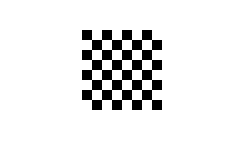
\includegraphics[width=\textwidth]{orig}
           \caption{Original}
           \label{fig:orig}
         \end{subfigure}
         \begin{subfigure}[b]{.16\textwidth}
           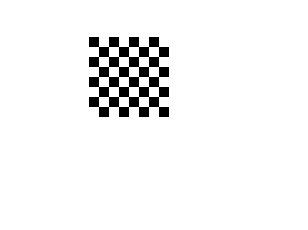
\includegraphics[width=\textwidth]{translate}
           \caption{Translate}
           \label{fig:trans}
          \end{subfigure}
          \begin{subfigure}[b]{.16\textwidth}
            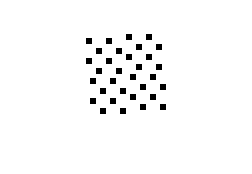
\includegraphics[width=\textwidth]{rotate}
            \caption{Rotate}
            \label{fig:rot}
          \end{subfigure}
          \begin{subfigure}[b]{.16\textwidth}
            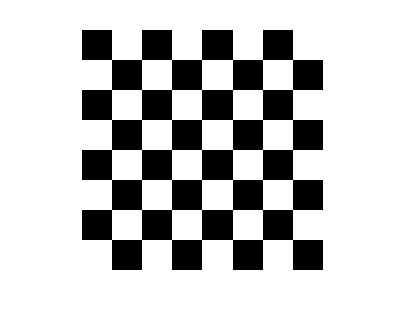
\includegraphics[width=\textwidth]{scale}
            \caption{Scale}
            \label{fig:scale}
          \end{subfigure}
          \begin{subfigure}[b]{.16\textwidth}
            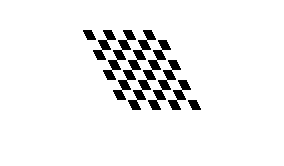
\includegraphics[width=\textwidth]{skew}
            \caption{Skew}
            \label{fig:skew}
          \end{subfigure}
          \begin{subfigure}[b]{.16\textwidth}
            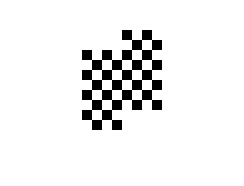
\includegraphics[width=\textwidth]{disjoint}
            \caption{Disjoint}
            \label{fig:disj}
          \end{subfigure}
          \caption{Artifical dataset}
          \label{fig:artificial}
       \end{figure}
       
       I was making a comparison between the different optical flow algorithms - Lucas-Kanade, Farnebäck, and Simpleflow - in order to be able to make an informed decision as to which one I would choose to continue to develop and work with for the remainder of the project. I compared the algorithms in terms of accuracy and speed. Speed is easily classified by measuring the time taken to process a frame of each of the videos. In order to ensure the reliability of the results, each test sequence was run three times, and the processing time was measured as an average across the three runs over the ten frames of each test video. Accuracy was measured qualitatively by comparing the output from the algorithms with prior knowledge of the motion in the test sequences. The test sequences were chosen as they each contain only one affine transformation, therefore making measuring the accuracy easier.
       
     \begin{figure}[h]
       \centering
        \begin{subfigure}[b]{.16\textwidth}
          \includegraphics[width=\textwidth]{{"../../experiments/sample sequences/translate.lucas-kanade.avi"}.png}
          \caption{Translate}
          \label{fig:translk}
        \end{subfigure}
        \begin{subfigure}[b]{.16\textwidth}
          \includegraphics[width=\textwidth]{{"../../experiments/sample sequences/rotate.lucas-kanade.avi"}.png}
          \caption{Rotate}
          \label{fig:rotlk}
        \end{subfigure}
        \begin{subfigure}[b]{.16\textwidth}
          \includegraphics[width=\textwidth]{{"../../experiments/sample sequences/scale.lucas-kanade.avi"}.png}
          \caption{Scale}
          \label{fig:scalelk}
        \end{subfigure}
        \begin{subfigure}[b]{.16\textwidth}
          \includegraphics[width=\textwidth]{{"../../experiments/sample sequences/skew.lucas-kanade.avi"}.png}
          \caption{Skew}
          \label{fig:skewlk}
        \end{subfigure}
        \begin{subfigure}[b]{.16\textwidth}
          \includegraphics[width=\textwidth]{{"../../experiments/sample sequences/fracture.lucas-kanade.avi"}.png}
          \caption{Disjoint}
          \label{fig:disjlk}
        \end{subfigure}
        \caption{Lucas-Kanade on Artificial Data}
        \label{fig:artificiallk}
      \end{figure}
      
      Figure~\ref{fig:artificiallk} shows the output of the optical flow algorithm for each of the test sequences. As the algorithm is a sparse optical flow algorithm it relies on a feature detector to select the points to track. In some cases, such as the skew in Figure~\ref{fig:skewlk}, the feature detector selects points which cluster around the centre of the frame and therefore provides suboptimal results.
      
      \begin{figure}[h]
        \centering
        \begin{subfigure}[b]{.16\textwidth}
          \includegraphics[width=\textwidth]{{"../../experiments/sample sequences/translate.farneback.avi"}.png}
          \caption{Translate}
          \label{fig:transfb}
        \end{subfigure}
        \begin{subfigure}[b]{.16\textwidth}
          \includegraphics[width=\textwidth]{{"../../experiments/sample sequences/rotate.farneback.avi"}.png}
          \caption{Rotate}
          \label{fig:rotfb}
        \end{subfigure}
        \begin{subfigure}[b]{.16\textwidth}
          \includegraphics[width=\textwidth]{{"../../experiments/sample sequences/scale.farneback.avi"}.png}
          \caption{Scale}
          \label{fig:scalefb}
        \end{subfigure}
        \begin{subfigure}[b]{.16\textwidth}
          \includegraphics[width=\textwidth]{{"../../experiments/sample sequences/skew.farneback.avi"}.png}
          \caption{Skew}
          \label{fig:skewfb}
        \end{subfigure}
        \begin{subfigure}[b]{.16\textwidth}
          \includegraphics[width=\textwidth]{{"../../experiments/sample sequences/fracture.farneback.avi"}.png}
          \caption{Disjoint}
          \label{fig:disjfb}
        \end{subfigure}
        \caption{Farnebäck on Artificial Data}
        \label{fig:artificialfb}
     \end{figure}
     
     Figure~\ref{fig:artificialfb} shows the output of the optical flow algorithm for each of the test sequences. Farnebäck optical flow is a dense optical flow algorithm, and therefore tracks all points from frame to frame. As a result it more accurately tracks the motion of the test sequences, even for a more difficult sequence such as Figure~\ref{fig:skewfb}.
     
     The SimpleFlow optical algorithm has a runtime two orders of magnitude slower than that of Farnebäck optical flow, and three orders of magnitude slower than Lucas-Kanade optical flow. This is most likely due to the algorithm being designed to be parallelised across many GPUs which are optimised to perform floating point operations. The speed of the algorithm therefore makes it practically unfeasible for use on the Raspberry Pi
           
      \begin{figure}[htbp!]
      \centering
        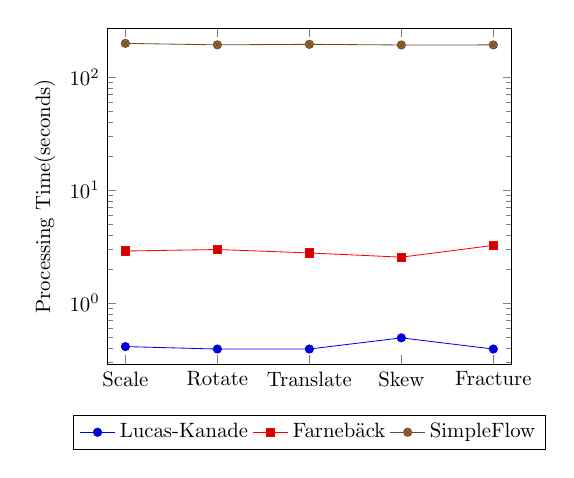
\begin{tikzpicture}[scale=0.75]
          \begin{semilogyaxis}[
            symbolic x coords={Scale,Rotate,Translate,Skew,Fracture},
            ylabel=Processing Time(seconds),
            enlargelimits=0.05,
            legend style={at={(0.5,-0.15)},
              anchor=north,legend columns=-1},
            ]
            \addplot
            coordinates {(Scale,0.41) (Rotate,0.39)
              (Translate,0.39) (Skew,0.49) (Fracture,0.39)};
            \addplot
            coordinates {(Scale,2.88) (Rotate,2.97)
              (Translate,2.77) (Skew,2.54) (Fracture,3.23)};
            \addplot
            coordinates {(Scale,198.97) (Rotate,193.01)
              (Translate,195.12) (Skew,192.52) (Fracture,192.82)};
            \legend{Lucas-Kanade,Farnebäck,SimpleFlow}
          \end{semilogyaxis}
        \end{tikzpicture}
        \label{fig:artitime}
        \caption{Processing Time Comparison}
      \end{figure}
      
      Figure 6 shows the processing time for each algorithm for each data set. Lucas-Kanade is consistently faster at processing than both Farnebäck and SimpleFlow. The only point of note is the result for the skew data set. the Lucas-Kanade algorithm processed the data set notably slower than the other data sets, whereas the Farnebäck algorithm processed the data set notably faster. There was no discernible difference for the SimpleFlow algorithm.
      
      Based on the above results, the Lucas-Kanade algorithm is consistently the fastest, and the Farnebäck algorithm is consistently the most accurate. The SimpleFlow algorithm provides no advantages on the Raspberry Pi hardware. Given that the speed difference between Lucas-Kanade and Farnebäck is small, I would suggest the Farnebäck algorithm 

    \subsection{Real World Data}
    
      In order to examine the algorithms in a real world scenario I was graciously provided with data sets from Dr Alexandre Kabla~\cite{harris2012characterizing}, my supervisor, and Mustafa Kamal, A PhD student in the Hopkinson Lab. Samples from both data sets can be seen in figure~\ref{fig:realworld}
      
      \begin{figure}[htbp!]
        \centering
        \begin{subfigure}[b]{0.3\textwidth}
          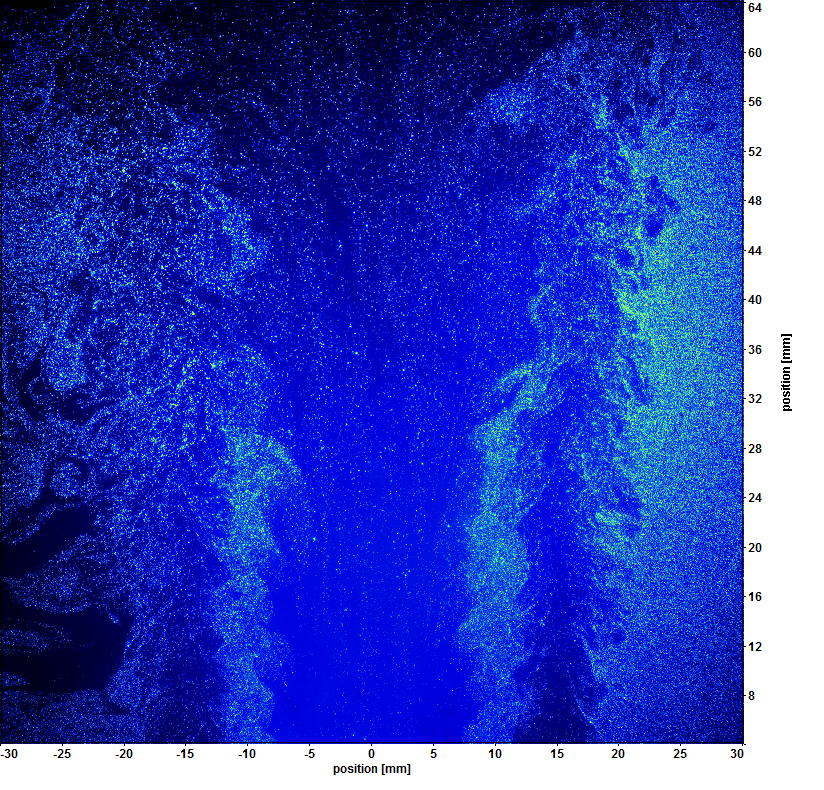
\includegraphics[width=\textwidth]{kamal}
          \caption{Data provided by Mustafa Kamal}
          \label{fig:kamal}
        \end{subfigure}
        \begin{subfigure}[b]{0.3\textwidth}
          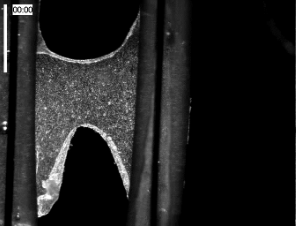
\includegraphics[width=\textwidth]{kabla}
          \caption{Data provided by Dr. Alexandre Kabla}
          \label{fig:kabla}
        \end{subfigure}
        \caption{Real world data sets used}
        \label{fig:realworld}
      \end{figure}
      
      I measured the average time to process a frame from each set using each algorithm. The results are plotted on a semi-log scale in figure~\ref{fig:realplot}.
    
      \begin{figure}[htbp!]
        \centering
        \begin{tikzpicture}[scale=0.75]
          \begin{axis}[legend entries={Lucas-Kanade, Farnebäck, SimpleFlow}, reverse legend, legend pos=outer north east,xlabel=Frame Size (MP),ylabel=Processing Time (seconds)
          ,ymode=log]
          \addplot table [x=a, y=LucasKanade, col sep=comma] {realworld.csv};
          \addplot table [x=a, y=Farneback, col sep=comma] {realworld.csv};
          \addplot table [x=a, y=SimpleFlow, col sep=comma] {realworld.csv};
          \end{axis}
        \end{tikzpicture}
        \caption{Processing time comparison}
        \label{fig:realplot}
      \end{figure}
      
      With regards to the usefulness of the output, while the Lucas-Kanade algorithm is consistently faster than the others, it is a sparse optical flow algorithm and therefore depends heavily on a separate feature detection algorithm to provide useful features to track. Some of the more popular algorithms include: the Harris edge detector~\cite{harris1988combined}, the Minimum Eigenvalues Algorithm~\cite{shi1994good} or the Canny Edge Detector~\cite{canny1986computational}. Obtaining information for key points may be useful for initial analysis of data, most use cases will require a full analysis of each frame. For this purpose only the Farnebäck algorithm is suitable.
      
      As can be seen in figure~\ref{fig:realplot} the SimpleFlow algorithm is approximately two orders of magnitude slower than the others. This is most likely due to the algorithm being designed for parallel processing, and the linear interpolation. The Raspberry Pi only has a single core ARM CPU, compared with high end GPUs which may have several thousand cores which can operate at several TFLOPs. The Lucas-Kanade algorithm is clearly the fastest algorithm, however it does not describe the entire flow. Despite the Farnebäck algorithm being slower than the Lucas-Kanade, it does provide us with a complete description of the flow, and for the reasons listed above I will recommend the Farnebäck optical flow algorithm.
      
  \section{Output}
  
    \subsection{Vector Arrows}
    
      In order to aid the visualisation of the vector field, I draw the vectors calculated from the optical flow methods. The method I wrote is similar to the MATLAB function \verb|quiver| in that it automatically scales the arrows depending on the magnitude of the vector. An example of the output can be seen in figure~\ref{fig:quiver}
      
      \begin{figure}[htbp!]
        \centering
        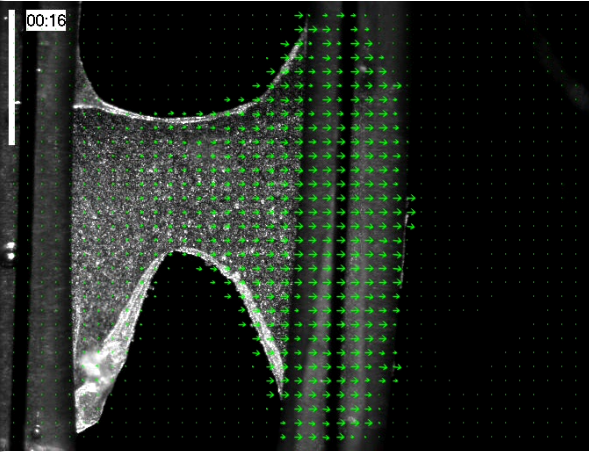
\includegraphics[width=.3\textwidth]{quiver}
        \caption{Vector arrows overlaid onto the data set}
        \label{fig:quiver}
      \end{figure}
    
    \subsection{Colour Map}
    
      The vector field can also be represented using a colour map. This is achieved by converting the cartesian vector coordinates into polar coordinates which are then mapped onto the HSV colour space as: Hue = Angle, Saturation = 255, Value = Magnitude. This can be seen in figure~\ref{fig:colour}
      
      \begin{figure}[htbp!]
        \centering
        \begin{subfigure}[b]{0.3\textwidth}
          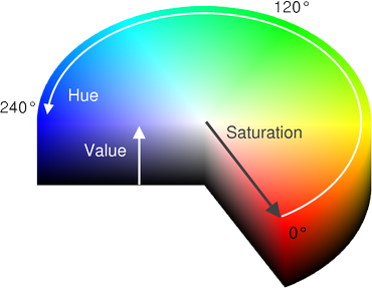
\includegraphics[width=\textwidth]{HSV}
          \caption{Mapping of vectors to HSV colour space}
          \label{fig:hsv}
        \end{subfigure}
        \begin{subfigure}[b]{0.3\textwidth}
          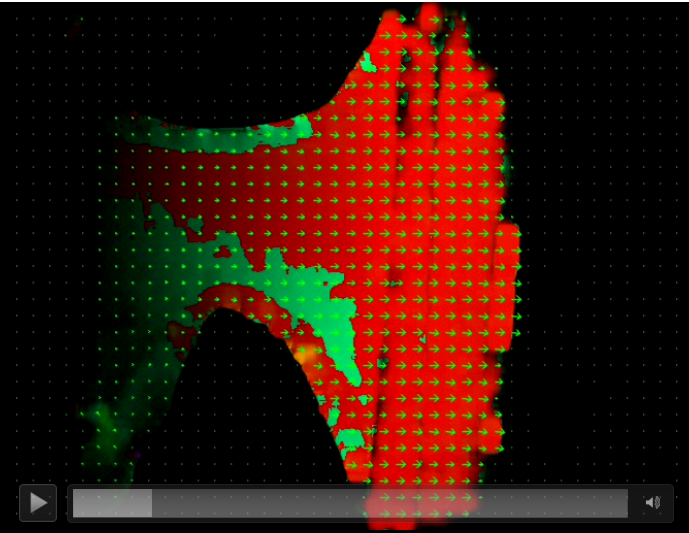
\includegraphics[width=\textwidth]{colour}
          \caption{An example mapping}
          \label{fig:colourmap}
        \end{subfigure}
        \caption{Mapping the vector field to the HSV colour space}
        \label{fig:colour}
      \end{figure}
      
  \section{Improvements}
  
    During lent term I would like to implement the curl and the divergence of the calculated vector field. If the vector field represents the flow velocity of a moving fluid, then the curl is the circulation density of the fluid and the divergence measures the magnitude of a vector field's source or sink at a given point. I will also optimise the implementation of my chosen optical flow algorithm in order to achieve as great performance as possible. This will lead onto integration with experiments, such as the 1st year materials testing lab. Finally, I will improve the user experience by providing a GUI for immediate user feedback.
      
  \section{References}
     
  \printbibliography[heading=none]
 
%  \section{Code Listings}
%  
%  \lstinputlisting[caption=How to setup OpenCV on the Raspberry Pi,label=lst:opencv]{"../install opencv.md"}
%  \lstinputlisting[language=C++,caption=Main optical flow method]{"../../experiments/comparison/optical-flow.cc"}
%  \lstinputlisting[language=C++,caption=Lucas-Kanade implementation in C++]{"../../experiments/comparison/lucas-kanade.cc"}
%  \lstinputlisting[language=C++,caption=Farnebäck implementation in C++]{"../../experiments/comparison/farneback.cc"}
%  \lstinputlisting[language=C++,caption=SimpleFlow implementation in C++]{"../../experiments/comparison/simpleflow.cc"}
%  \lstinputlisting[language=MATLAB,caption=MATLAB code to generate sample sequences,label=lst:generate]{"../../experiments/sample sequences/generate.m"}

%    
\end{document}